\documentclass[
  11pt,
  letterpaper,
   addpoints,
   answers
  ]{exam}

\usepackage{../exercise-preamble}
\usepackage{amsmath} % matrices (pmatrix, vmatrix), etc.
\usepackage{bm}      % \bm{·} para negrita en modo matemático
\usepackage{float}
\usepackage{graphicx}

\begin{document}
% Override preamble's \pagestyle{empty}: show page numbers centered in the footer
\pagestyle{headandfoot}
\firstpageheader{}{}{}
\runningheader{}{}{}
\firstpagefooter{}{\thepage}{}
\runningfooter{}{\thepage}{}

\noindent
\begin{minipage}{0.47\textwidth}

\includegraphics[width=\textwidth]{../fcfm_die}
\end{minipage}
\begin{minipage}{0.53\textwidth}
\begin{center}
\large\textbf{Análisis de Sistemas Dinámicos y Estimación} (EL3204-1) \\
\large\textbf{Clase auxiliar 4} \\
\normalsize Prof.~ Marcos Orchard - Sebastián Espinosa.\\
\normalsize Prof.~Aux.~Erik Sáez
\end{center}
\end{minipage}

\vspace{0.5cm}
\noindent
\vspace{.85cm}

\begin{questions}
    %%%%%%%%%%%%%%%%%%%%%%%%%%%
  \question Considere el sistema en tiempo continuo dado por
  \begin{equation}
      \ddot y(t) - 2\dot y(t) - 8 y(t) = 3\dot u(t) + 3 u(t),
      \label{eq:plant}
  \end{equation}
  donde $u(t)$ es la entrada y $y(t)$ la salida.

  \begin{parts}
    \part Obtenga la función de transferencia $G(s)=\dfrac{Y(s)}{U(s)}$ del sistema (condiciones iniciales nulas).
    \part A partir de $G(s)$, proponga una representación en espacio de estados $(\dot x = Ax + Bu,\; y = Cx + Du)$ en forma controlable.
    \part Determine si el sistema es controlable y observable. Justifique mediante los rangos de las matrices de controlabilidad y observabilidad.
    \part Diseñe un controlador por realimentación de estados $u = -Kx + r$ que ubique los polos a lazo cerrado en $s=-5$ y $s=-3$. Indique el vector $K$.
    \part Suponga ahora que sólo se mide la salida $y(t)$ y no el estado completo. Diseñe un compensador dinámico (controlador con observador de estado) que mantenga los polos de lazo cerrado en $-5$ y $-3$. Indique los polos del observador y el vector de ganancias $L$.
  \end{parts}
  % Comienzo de soluciones dentro del entorno questions
\begin{solution}
  \subsection*{Resolución 1.1}
  Dado que estamos trabajando en el dominio temporal continuo, pasamos al dominio de Laplace. Aplicando transformada de Laplace (CI nulas) a \eqref{eq:plant}:
  \begin{align}
      s^2 Y(s) - 2s Y(s) - 8 Y(s) &= 3s U(s) + 3 U(s) \nonumber \\
      (s^2 - 2s - 8)Y(s) &= (3s + 3)U(s). \label{eq:plant_laplace}\\
      \Longrightarrow \quad G(s)=\frac{Y(s)}{U(s)} &= \frac{3s+3}{s^{2}-2s-8}. \nonumber
  \end{align}
Luego debemos aplicar fracciones parciales para escribir $G(s)$ como suma de términos simples. Factorizamos el denominador: $s^{2}-2s-8 = (s-4)(s+2)$. Usamos fracciones parciales
\begin{align}
      G(s)=\frac{\alpha}{s-4}+\frac{\beta}{s+2} = \frac{\alpha(s+2)+\beta(s-4)}{(s-4)(s+2)}= \frac{3s+3}{(s-4)(s+2)}
\end{align}
De esta manera tenemos el siguiente sistema de ecuaciones para el numerador:
\begin{align}
  \alpha(s+2)+\beta(s-4) &= 3s+3 \nonumber \\
  (\alpha+\beta)s + (2\alpha - 4\beta) &= 3s + 3 \nonumber \\
\end{align}
De esta manera tenemos que:
\begin{align}
  \alpha + \beta &= 3 \label{eq:sistema1} \\
  2\alpha - 4\beta &= 3 \label{eq:sistema2}
\end{align}
Con lo que finalmente se tiene que $\alpha = \tfrac{5}{2}$ y $\beta = \tfrac{1}{2}$. Por lo tanto:
\begin{align}
  G(s) = \left(\frac{5}{2}\right)\frac{1}{s-4} + \left(\frac{1}{2}\right)\frac{1}{s+2}
\end{align}
Así se obtiene la función de transferencia del sistema.

  \subsection*{Resolución 1.2}
Recordando que es posible escribir $G(s)= \frac{Y(s)}{U(s)}$, la salida será:
\begin{align}
      Y(s) = G(s)U(s) = \frac{3s+3}{s^{2}-2s-8}U(s) = \left(\frac{5}{2}\right)\frac{U(s)}{s-4} + \left(\frac{1}{2}\right)\frac{U(s)}{s+2}
\end{align}
De esta manera es posible escribir el vector $C$ de forma conveniente dada por:
\begin{align}
  Y(s) = (1 \quad 1) \begin{pmatrix} \left(\frac{5}{2}\right)\frac{U(s)}{s-4} \\ \left(\frac{1}{2}\right)\frac{U(s)}{s+2} \end{pmatrix}
\end{align}
Notar que tambien podriamos formularlo como:
\begin{align}
  Y(s) = \begin{pmatrix} \frac{5}{2} & \frac{1}{2}\end{pmatrix} \begin{pmatrix} \frac{U(s)}{s-4} \\ \frac{U(s)}{s+2} \end{pmatrix}
\end{align}
Es equivalente dado que los polos nos damos que unicamente se ponderan pero no cambian su valor, por lo que la estabilidad no se ve afectada. En este caso se escoge la primer forma. Definiendo:
\begin{align}
  C= \begin{pmatrix} 1 & 1 \end{pmatrix}, \quad X(s) = \begin{pmatrix} X_1(s) \\ X_2(s) \end{pmatrix} = \begin{pmatrix} \left(\frac{5}{2}\right)\frac{U(s)}{s-4} \\ \left(\frac{1}{2}\right)\frac{U(s)}{s+2} \end{pmatrix}
\end{align}
De esta manera tendremos que:
\begin{align}
  X_1(s) = \left(\frac{5}{2}\right)\frac{U(s)}{s-4} \quad &\Longrightarrow \quad sX_1(s) - 4X_1(s) = \left(\frac{5}{2}\right)U(s) \quad \Longrightarrow \quad \dot{x}_1(t) = 4x_1(t) + \left(\frac{5}{2}\right)u(t) \\
\end{align}
Análogamente, para $X_2(s)$:
\begin{align}
  X_2(s) = \left(\frac{1}{2}\right)\frac{U(s)}{s+2} \quad &\Longrightarrow \quad sX_2(s) + 2X_2(s) = \left(\frac{1}{2}\right)U(s) \quad \Longrightarrow \quad \dot{x}_2(t) = -2x_2(t) + \left(\frac{1}{2}\right)u(t)
\end{align}
Con lo que finalmente es posible formular la representación en espacio de estados del sistema como:
\begin{align}
  \dot{x}_1(t) &= 4x_1(t) + \left(\frac{5}{2}\right)u(t) \\
  \dot{x}_2(t) &= -2x_2(t) + \left(\frac{1}{2}\right)u(t) \\
\end{align}
Donde en forma matricial se tendra que:
\begin{align}
  \begin{pmatrix}
    \dot{x}_1(t) \\ \dot{x}_2(t)
  \end{pmatrix}
  &=
  \begin{pmatrix}
    4 & 0 \\
    0 & -2
  \end{pmatrix}
  \begin{pmatrix}
    x_1(t) \\ x_2(t)
  \end{pmatrix}
  +
  \begin{pmatrix}
   5/2 & 1/2
  \end{pmatrix}
  u(t) 
\end{align}

Donde reconocemos las matrices $A$ y $B$ dadas por:
\begin{align}
  A &= \begin{pmatrix}
    4 & 0 \\
    0 & -2
  \end{pmatrix}, \quad
  B = \begin{pmatrix}
    5/2 \\ 1/2
  \end{pmatrix}
\end{align}

Por otro lado, tendremos que la salida del sistema será:
\begin{align}
  y(t) &= \begin{pmatrix} 1 & 1 \end{pmatrix} \begin{pmatrix} x_1(t) \\ x_2(t) \end{pmatrix} + 0 \cdot u(t) \\
  &= \begin{pmatrix} 1 & 1 \end{pmatrix} x(t) 
\end{align}
  

  \subsection*{Resolución 1.3}
Recordemos que para determinar si un sistema es controlable u observable, debemos calcular las matrices de controlabilidad y observabilidad respectivamente y luego determinar sus rangos. La matriz de controlabilidad viene dada por:
\begin{align}
  \mathcal C = \begin{pmatrix} B & AB & A^2B & \cdots & A^{n-1}B \end{pmatrix}
\end{align}
Que para nuestro caso particular tenemos que $n=2$, por lo que:
\begin{align}
  \mathcal C = \begin{pmatrix} B & AB \end{pmatrix}
\end{align}
Luego, calculamos $AB$:
\begin{align}
  AB = A \cdot B = \begin{pmatrix} 4 & 0 \\ 0 & -2 \end{pmatrix} \cdot \begin{pmatrix} 5/2 \\ 1/2 \end{pmatrix} = \begin{pmatrix} 4 \cdot (5/2) + 0 \cdot (1/2) \\ 0 \cdot (5/2) + (-2) \cdot (1/2) \end{pmatrix} = \begin{pmatrix} 10 \\ -1 \end{pmatrix}
\end{align}
Por lo que finalmente tenemos que:
\begin{align}
  \mathcal C = \begin{pmatrix} B & AB \end{pmatrix} = \begin{pmatrix} 5/2 & 10 \\ 1/2 & -1 \end{pmatrix}
\end{align}
Vemos que la matriz es Linealmente independiente tanto en columnas como en filas, por lo que su rango es 2. Por lo tanto el sistema es controlable. Otra forma de verificar esto es calculando el determinante de la matriz y este debe ser diferente de cero. Calculamos:
\begin{align}
  \det(\mathcal C) = \left( \frac{5}{2} \cdot (-1) \right) - (10 \cdot \frac{1}{2}) = -\frac{5}{2} - 5 = -\frac{15}{2} \neq 0
\end{align}
Por lo que el sistema es controlable. Luego analizamos la matriz de observabilidad, la cual viene dada por:
\begin{align}
  \mathcal O = \begin{pmatrix} C \\ CA \\ CA^2 \\ \vdots \\ CA^{n-1} \end{pmatrix}
\end{align}
Que para nuestro caso particular tenemos que $n=2$, por lo que:
\begin{align}
  \mathcal O = \begin{pmatrix} C \\ CA \end{pmatrix}
\end{align}
Calculamos $CA$:
\begin{align}
  CA = C \cdot A = \begin{pmatrix} 1 & 1 \end{pmatrix} \cdot \begin{pmatrix} 4 & 0 \\ 0 & -2 \end{pmatrix} = \begin{pmatrix} 1 \cdot 4 + 1 \cdot 0 & 1 \cdot 0 + 1 \cdot (-2) \end{pmatrix} = \begin{pmatrix} 4 & -2 \end{pmatrix}
\end{align}
Por lo que finalmente tenemos que:
\begin{align}
  \mathcal O = \begin{pmatrix} C \\ CA \end{pmatrix} = \begin{pmatrix} 1 & 1 \\ 4 & -2 \end{pmatrix}
\end{align}
Nuevamente vemos que la matriz es Linealmente independiente tanto en columnas como en filas, por lo que su rango es 2. Por lo tanto el sistema es observable. Otra forma de verificar esto es calculando el determinante de la matriz y este debe ser diferente de cero. Calculamos:
\begin{align}
  \det(\mathcal O) = (1 \cdot (-2)) - (1 \cdot 4) = -2 - 4 = -6 \neq 0
\end{align}
Por lo que el sistema es observable.
  \subsection*{Resolución 1.4}
  Dado que verificamos previamente que el sistema es controlable, podemos proceder a diseñar un controlador por realimentación de estados. La ley de control es $u = r - Kx$, donde $r$ es la referencia (aquí se asume constante) y $K$ es el vector de ganancias a determinar. El sistema en lazo cerrado queda
  Se busca $K$ tal que los polos de $A-BK$ estén en $-5$ y $-3$. Esta metodología se utiliza porque anteriormente obtuvimos que los polos del sistema eran $4$ y $-2$; el 4 es positivo y produce inestabilidad. Mediante esta realimentación se busca estabilizar el sistema. El sistema original se puede ver mediante el diagrama de bloques:
  \begin{figure}[H]\centering
    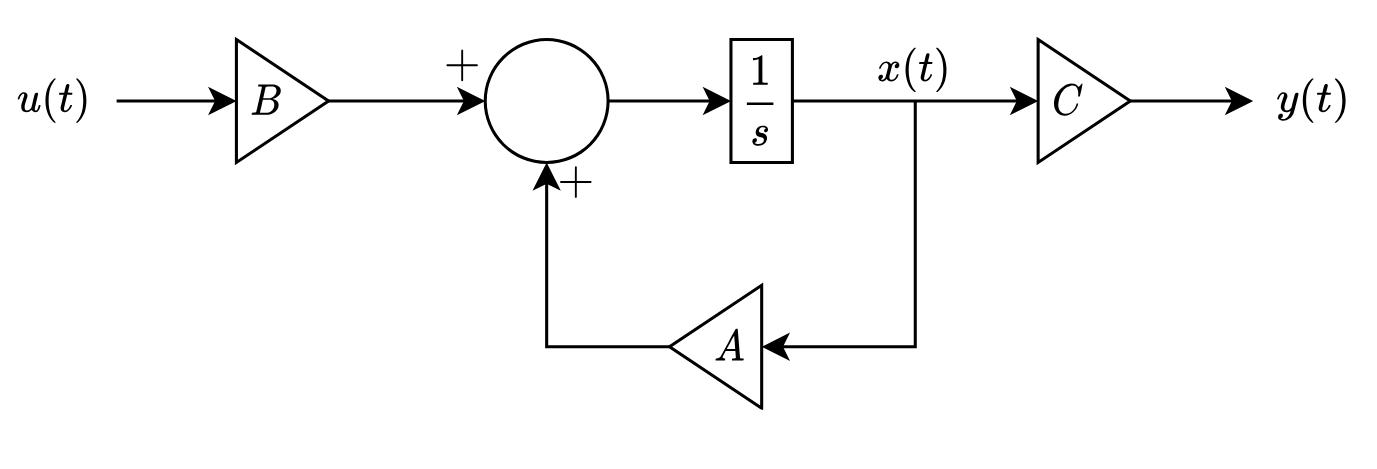
\includegraphics[width=.9\textwidth]{../figures/Auxiliar_4_1.png}
    \caption{El diagrama muestra la estructura estándar de un sistema lineal en espacio de estados: la entrada $u(t)$ es multiplicada por $B$ y sumada al término asociado a la dinámica interna $Ax(t)$ antes de integrarse (bloque $\tfrac{1}{s}$ que representa $\int$) para generar el estado $x(t)$. La salida se obtiene aplicando $C$ a $x(t)$. La realimentación con $A$ en el lazo interno ilustra simbólicamente la contribución de la dinámica interna $Ax$ al acumulador. De manera conceptual, cada rama representa uno de los componentes del estado $x(t)$.}
  \end{figure} 
Por otro lado, dado que ajustaremos la entrada $u$ mediante la realimentación de estados, el sistema en lazo cerrado se puede ver como:
 \begin{figure}[H]\centering
    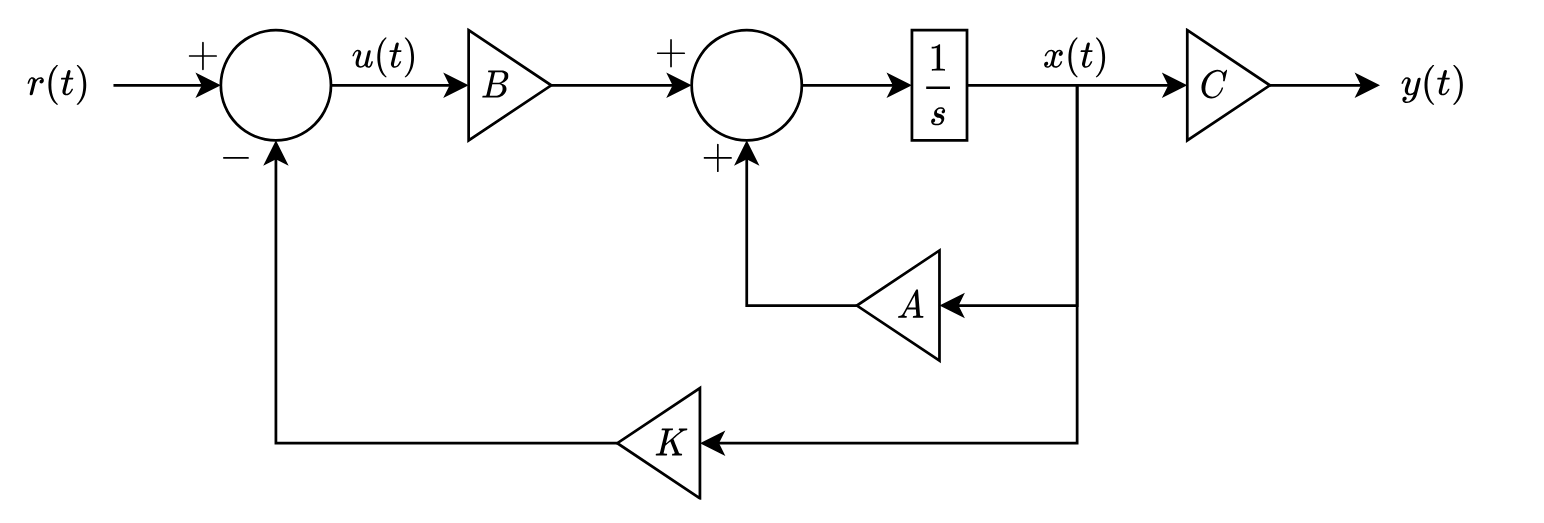
\includegraphics[width=.9\textwidth]{../figures/Auxiliar_4_2.png}
    \caption{El bloque punteado corresponde al observador que genera $\hat x(t)$ a partir de $u(t)$ y $y(t)$. La señal de innovación $e_y(t)= y(t)-\hat y(t)$ (comparador a la derecha) se amplifica por $F$ y se inyecta en la misma estructura dinámica $(A, B)$ que replica el modelo interno. Esto corrige continuamente la estimación: si $\hat y$ es menor que $y$, el término $F e_y$ empuja la trayectoria estimada en la dirección adecuada. Afuera del bloque, el controlador usa la estimación (en lugar del estado real) para formar la acción $u = r - K\hat x$.}
  \end{figure}
  Volviendo sobre nuestra representación en espacio de estados, tenemos:
  \begin{align}
      \dot x &= Ax + Bu = Ax + B(r - Kx) = (A-BK)x + Br \\
      y &= Cx + Du = Cx + 0(r - Kx) = Cx
  \end{align}
  Por lo que el sistema en lazo cerrado queda $\dot x = (A-BK)x + Br$, $y = Cx$. La estabilidad del sistema en lazo cerrado está dada por los autovalores de $A-BK$ que denominaremos $\hat{A}$, notamos que el vector K es de la forma $K = (k_1 \; k_2)$, y al ser una variable libre podemos elegir sus valores para ubicar los polos de $\hat{A}$ en las posiciones deseadas., por lo tanto se obtienen primeramente los polos dados por:
  \begin{align}
    \det(A-BK -\lambda I) &= 0\\
    \lambda^{2} + \left(-2 + \frac{5}{2}k_1 + \frac{1}{2}k_2\right)\lambda + \left(-8 + 5k_1 - 2k_2\right) &= 0
  \end{align}
  Estos valores obtenidos deben ser iguales a los polos deseados, que en este caso son $-5$ y $-3$. Por lo que el polinomio característico deseado es:
  \begin{align}
    (\lambda + 5)(\lambda + 3) = \lambda^{2} + 8\lambda + 15
  \end{align}
  Igualando los coeficientes de ambos polinomios, se obtiene el siguiente sistema de ecuaciones:
  \begin{align}
    -2 + \frac{5}{2}k_1 + \frac{1}{2}k_2 &= 8 \\
    -8 + 5k_1 - 2k_2 &= 15
  \end{align}
  Resolviendo el sistema de ecuaciones, se obtiene que $k_1 = \frac{21}{5}$ y $k_2 = -1$. Por lo tanto, el vector de ganancias $K$ es:
  \begin{align}
    K = \left( \frac{21}{5} \; -1 \right)
  \end{align}
  Con lo que finalmente vemos el vector de ganancias $K$ que ubica los polos del sistema en lazo cerrado en $-5$ y $-3$. La ley de control es $u = r - Kx$.

  \subsection*{Resolución 1.5}
  En el análisis que sigue debemos cuidar la idea central que se quiere transmitir. Ahora no tenemos acceso al estado completo, sólo a la salida $y$. La pregunta natural es: ¿cómo estimar $x$ a partir de $y$? La respuesta es usar un observador de estados. El observador de Luenberger replica la dinámica del sistema original e incorpora la información de la salida medida para corregir la estimación. Se diseña de modo que el error entre el estado real y el estimado converge a cero con el tiempo, garantizando una estimación precisa. Matemáticamente:
  \begin{align}
    \dot{\hat x} &= A\hat x + Bu + F(y - \hat y) \\
    \hat y &= C\hat x
  \end{align}
  Donde $\hat x$ es la estimación del estado, $\hat y$ es la salida estimada, y $F$ es el vector de ganancias del observador a determinar. Esto, en un diagrama de bloques, se observa como:
    \begin{figure}[H]\centering
    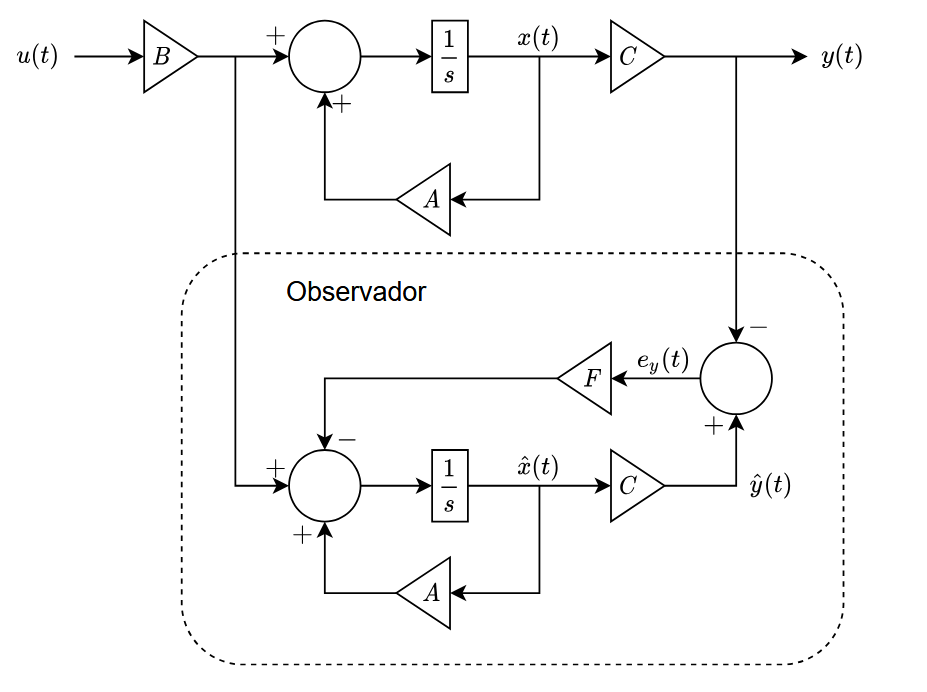
\includegraphics[width=.9\textwidth]{../figures/Auxiliar_4_3.png}
    \caption{El observador replica la ecuación $\dot{\hat x}=A\hat x + Bu + F(y-\hat y)$. La rama principal implementa el modelo del sistema ($A$, $B$ y el integrador). La rama vertical superior lleva la salida estimada $\hat y = C\hat x$ al comparador donde se obtiene el error de salida $e_y$. Ese error, tras el bloque de ganancia $F$, se suma como término corrector que desplaza los polos de la dinámica del error a posiciones elegidas (más rápidos), garantizando convergencia de $\hat x$ hacia $x$. De este modo el diseño de $F$ es independiente del de $K$, ilustrando el principio de separación.}
  \end{figure}
El error estará dado por:
  \begin{align}
    e = \hat x - x
  \end{align}
  Y su dinámica estará dada por:
  \begin{align}
    \dot{e}(t) =& A\hat{x(t)} + Bu(t) + F(y(t) - \hat{y}(t)) - (Ax(t) + Bu(t)) \\
    =& A(\hat{x(t)} - x(t)) + F(Cx(t) - C\hat{x(t)})\\
     &= (A - FC)e(t)
  \end{align}
  La dinámica del error depende de la matriz $A - FC$. Para garantizar que el error converja a cero es necesario que los autovalores de $A - FC$ tengan parte real negativa. Esto se logra eligiendo adecuadamente $F$. Como el sistema es observable podemos ubicar los polos de $A - FC$ libremente. Usualmente se eligen más rápidos ( tres veces más negativos) que los del controlador para asegurar convergencia rápida. Procedemos a calcular $F$ para ubicar polos en $-15$ y $-9$. Sea
  \begin{align}
    F = \begin{pmatrix} f_1 \\ f_2 \end{pmatrix}
  \end{align}
  Lo que permite que obtener los polos de la matriz como:
  \begin{align}
    \det(sI - (A - FC)) = \lambda^{2} - (2 - (f_1 + f_2))\lambda + (-8 + 2f_1 - 4f_2) = 0
  \end{align}
  De esta manera dado que queremos ubicar los polos en $-15$ y $-9$, el polinomio característico deseado es:
  \begin{align}
    (\lambda + 15)(\lambda + 9) = \lambda^{2} + 24\lambda + 135
  \end{align}
  Igualando los coeficientes de ambos polinomios, se obtiene el siguiente sistema de ecuaciones:
  \begin{align}
    -(2 - (f_1 + f_2)) &= 24 \\
    -8 + 2f_1 - 4f_2 &= 135
  \end{align}
  Resolviendo el sistema de ecuaciones, se obtiene que $f_1 = \frac{247}{6}$ y $f_2 = -\frac{91}{6}$. Por lo tanto, el vector de ganancias $F$ es:
  \begin{align}
    F = \begin{pmatrix} \frac{247}{6} \\ -\frac{91}{6} \end{pmatrix}
  \end{align}
  % Explicación ampliada del principio de separación
  \paragraph{Principio de separación (explicación).} El controlador por realimentación de estados diseña $K$ para colocar los polos de la matriz $A-BK$. Cuando agregamos un observador de Luenberger, la dinámica conjunta (control + observador) en las coordenadas $x$ (estado real) y $e = \hat x - x$ (error de estimación) queda
  \[
     \dot x = (A-BK)x + Br, \qquad \dot e = (A-FC)e.
  \]
  Obsérvese que $e$ no aparece en la ecuación de $\dot x$ (no hay términos cruzados). Esto significa que la evolución del estado real (y, por ende, del lazo de control) no depende de cómo transcurre transitoriamente el error del observador: mientras $K$ estabilice/ubique los polos deseados de $(A-BK)$, esa parte permanecerá válida. En paralelo, $F$ se elige para que $(A-FC)$ haga que $e(t)\to 0$ rápidamente. Así, el diseño se separa en dos problemas independientes: (i) colocación de polos de control y (ii) colocación de polos del observador.
  
  En términos más formales, si el par $(A,B)$ es estabilizable y el par $(A,C)$ es detectable (en nuestro caso son controlable y observable, condiciones más fuertes), entonces existe una elección de $K$ y $F$ tal que ambos subsistemas son estables y la matriz bloque triangular
  \[
     \begin{pmatrix} A-BK & -BK \\ 0 & A-FC \end{pmatrix}
  \]
  tiene autovalores exactamente iguales a la unión de los autovalores de $A-BK$ y $A-FC$. Por eso podemos reutilizar, sin modificaciones, el $K$ calculado en la Parte 4 incluso cuando sólo disponemos de $\hat x$: basta sustituir $x$ por $\hat x$ en la ley de control $u = r - K\hat x$. Una vez que $e(t)$ converge a cero, $\hat x \approx x$ y la acción de control coincide prácticamente con la que se habría aplicado con estado completo. El beneficio de elegir polos del observador más rápidos (más a la izquierda) es minimizar el impacto transitorio de los errores de estimación sobre la salida.
  \end{solution}
%----------------------------  Segunda pregunta
  \question Considere un motor eléctrico DC que impulsa un carrito, como se muestra en la figura.
  \begin{center}
    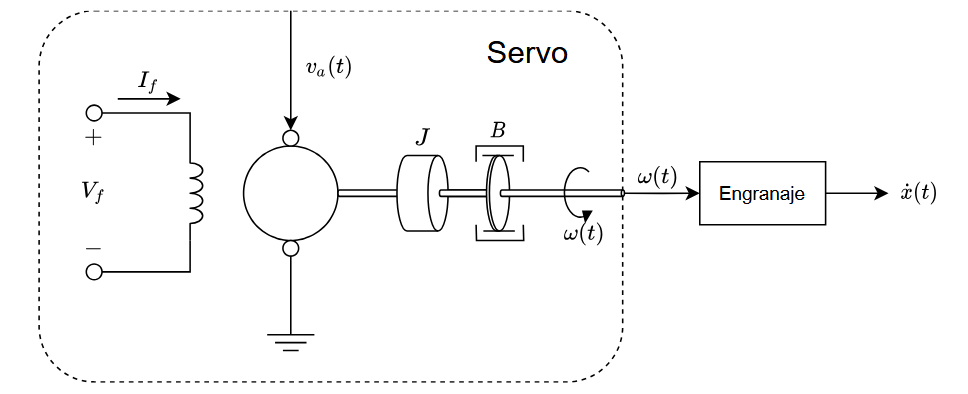
\includegraphics[width=.75\textwidth]{../figures/Auxiliar_4_4.png}
  \end{center}
  Suponga que los parámetros del sistema son:
  \[
     k_m = 1\;\text{Nm/A},\quad k_e = 1\;\text{Vs},\quad R_a = 0.01\,\Omega,\quad L_a = 1\,\text{H},        \\
     J = 0.1\,\text{kgm}^2,\quad B = 0.2\,\text{Nms}, \quad k_g = 0.01\,\text{m/rad}.
  \]
  \begin{parts}
    \part Formule un modelo dinámico del sistema en variables de estado, indicando claramente las hipótesis simplificatorias (por ejemplo: juego de engranajes ideal, sin pérdidas; fricción viscosa lineal; flujo magnético constante, etc.).
    \part Encuentre la función de transferencia (MTE) desde el voltaje de armadura $v_a(t)$ hasta la velocidad lineal $\dot z(t)$ del carrito.
    \part Determine si el sistema es estable (según los polos de la MTE / matriz $A$).
    \part Obtenga la respuesta al impulso de la salida $\dot z(t)$.
    \part Exprese la respuesta del sistema en un tiempo arbitrario $t$ para condiciones iniciales y entrada arbitraria (solución general usando convolución o solución de estado).
    \part Determine si el sistema es completamente controlable y observable (especifique la elección de estados utilizada).
    \part En caso de ser observable, diseñe un observador cuyos polos se ubiquen en $-10$ y $-5$.
  \end{parts}
% (Sin solución incluida para esta pregunta de momento.)
\end{questions}
\begin{solution}
\subsection*{Resolución 2.2}
Suponiendo una carga fija podemos modelar el rotor de la siguiente manera:
\begin{figure}[H]
\centering
\begin{circuitikz}[american voltages, european resistors]
  \draw
    (0,0) to[sV, l_={$v_a(t)$}] (0,3)    % fuente de armadura
           to[R,  l={$R_a$}]     (3,3)    % resistencia
           to[L,  l={$L_a$}]     (6,3)    % inductancia
           to[V,  l_={$e(t)=k_e\,\omega(t)$}] (6,0) % fem de retroceso (+ arriba)
           -- (0,0);                        % cierre del lazo

  % Anotamos la corriente de armadura encima del resistor (opcional)
  \draw[->] (3.3,3.25) -- (3.8,3.25) node[midway, above] {$i_a(t)$};
\end{circuitikz}
\caption{Modelo eléctrico de la armadura con $e(t)=k_e\,\omega(t)$.}
\label{fig:armadura}
\end{figure}

El modelo eléctrico de la armadura, mostrado en la Fig.~\ref{fig:armadura}, se obtiene por ley de mallas:
\begin{align}
V_{a}&= R_{a}i_{a} + V_L + k_e \omega(t)\\ 
V_a&=-R_a\,i_a(t)+L_a\,\frac{di_a(t)}{dt}+k_e\,\omega(t).\\
\frac{\partial i_a(t)}{\partial t} &= -\frac{R_a}{L_a}\,i_a(t)-\frac{k_e}{L_a}\,\omega(t)+\frac{1}{L_a}\,v_a(t).
\end{align}
Por otro parte, para la parte mecanica, sabemos $\tau = k_m\,i_a(t)$. por lo tanto:
\begin{align}
\tau_m = \sum_{i} \tau_i 
\end{align}
De esta manera por ley de torques tenemos que $J \dot{\omega}$ por inercia y $B \omega$ por roce, de esta manera tenemos que:
\begin{align}
  k_m\,i_a(t)&=J\,\dot{\omega}(t)+B\,\omega(t).\\
  \dot{\omega}(t)&=-\frac{B}{J}\,\omega(t)+\frac{k_m}{J}\,i_a(t).
\end{align}
Luego tomamos las dos ecuaciones diferenciales obtenidas y las ordenamos:
\begin{align}
 \frac{\partial \omega(t)}{\partial t} &= -\frac{B}{J}\,\omega(t)+\frac{k_m}{J}\,i_a(t),\\
  \frac{\partial i_a(t)}{\partial t} &= -\frac{R_a}{L_a}\,i_a(t)-\frac{k_e}{L_a}\,\omega(t)+\frac{1}{L_a}\,v_a(t).
\end{align}
Luego podemos definir el vector de estado y la entrada como:
\begin{equation}
  x(t)=\begin{bmatrix}\omega(t)\\ i_a(t)\end{bmatrix},
  \qquad
  u(t)=v_a(t).
\end{equation}
De esta manera podemos observar que el sistema queda en la forma estandar de espacio de estados donde las matrices $A$ y $B$ quedan definidas como:
\begin{equation}
  \dot{x}(t)=
  \underbrace{\begin{bmatrix}
    -\dfrac{B}{J} & \dfrac{k_m}{J}\\[6pt]
    -\dfrac{k_e}{L_a} & -\dfrac{R_a}{L_a}
  \end{bmatrix}}_{A}\,x(t)
  +
  \underbrace{\begin{bmatrix}
    0\\[2pt]\dfrac{1}{L_a}
  \end{bmatrix}}_{B}\,u(t).
\end{equation}
La salida requerida es la velocidad lineal del carrito, proporcional a la velocidad angular del eje:
\begin{align}
  y(t)=\dot z(t)=k_g\,\omega(t)
  =&
  \underbrace{\begin{bmatrix}k_g & 0\end{bmatrix}}_{C}\,x(t)
  +
  \underbrace{0}_{D}\,u(t).\\
  =&\begin{bmatrix}
    k_g & 0
  \end{bmatrix}
  \begin{bmatrix}
    \omega(t)\\ i_a(t)
  \end{bmatrix}
\end{align}
Algunas hipótesis simplificatorias podrían ser:
\begin{itemize}
  \item Juego de engranajes ideal, sin pérdidas.
  \item Fricción viscosa lineal.
  \item Flujo magnético constante.
  \item No hay saturación magnética.
  \item El motor opera en su región lineal.
  \item El carrito se mueve en una superficie horizontal sin pendiente.
  \item No hay fuerzas externas actuando sobre el carrito (como viento o fricción adicional).
  \item $\ddots$
\end{itemize}
\subsection*{Resolucion 2.1}

Con los parámetros usados en el desarrollo manuscrito
$k_m=1$, $k_e=1$, $R_a=1~\Omega$, $L_a=1~\mathrm{H}$, $J=0.1~\mathrm{kg\,m^2}$,
$B=0.2~\mathrm{N\,m\,s}$ y $k_g=0.01~\mathrm{m/rad}$, el modelo queda

\begin{align}
A&=
\begin{bmatrix}
-\dfrac{B}{J} & \dfrac{k_m}{J}\\[4pt]
-\dfrac{k_e}{L_a} & -\dfrac{R_a}{L_a}
\end{bmatrix}
=
\begin{bmatrix}
-2 & 10\\
-1 & -1
\end{bmatrix},\qquad
B=
\begin{bmatrix}
0\\[2pt] \dfrac{1}{L_a}
\end{bmatrix}
=
\begin{bmatrix}
0\\ 1
\end{bmatrix},\qquad
C=\begin{bmatrix} k_g & 0\end{bmatrix}=\begin{bmatrix}0.01 & 0\end{bmatrix}.
\end{align}
Notamos que la matriz $A$ no es diagonal, pero si es diagonalizable dado que es de rango completo, por lo que planteamos que $A=TDT^{-1}$, donde $D$ es diagonal y $T$ es la matriz de autovectores. Por lo tanto el polinomio característico de $A$ vendra dado por:
\begin{align}
\det(\lambda I-A)=(\lambda+2)(\lambda+1)+10
=\lambda^2+3\lambda+12.
\end{align}
De esta manera definimos que:
\begin{align}
  \lambda_1 &= -1.5 + j\frac{\sqrt{39}}{2}\\ \lambda_2 &= -1.5 - j\frac{\sqrt{39}}{2}
\end{align}
Luego, definimos la matriz $D$ como la matriz diagonal formada por los autovalores:
\begin{equation}
  D = \begin{pmatrix} \lambda_1 & 0 \\ 0 & \lambda_2 \end{pmatrix} = \operatorname{diag}(\lambda_1,\lambda_2).
\end{equation}
Luego, para obtener un autovector asociado a $\lambda_1$ resolvemos
\begin{align}
  (A- \lambda_1 I)v_1 = 0 \;\Longrightarrow\;
  \begin{bmatrix}
    -2 -(-1.5 + j\dfrac{\sqrt{39}}{2}) & 10 \\
    -1 & -1 -(-1.5 + j\dfrac{\sqrt{39}}{2})
  \end{bmatrix}
  \begin{bmatrix}
    v_{x1} \\ v_{y1}
  \end{bmatrix}
  = \begin{bmatrix}
    0 \\ 0
  \end{bmatrix}
\end{align}
Luego tenemos que resolviendo:
\begin{align}
  \left(-0.5 - j\frac{\sqrt{39}}{2}\right)v_{x1} + 10 v_{y1} &= 0 \\
  -v_{x1} + \left(0.5 - j\frac{\sqrt{39}}{2}\right)v_{y1} &= 0
\end{align}
Tomando $v_{x1}=1$ se obtiene $v_{y1} = 0.05 + j\tfrac{\sqrt{39}}{20}$, dando como resultado el vector:
\begin{align}
  v_1 = \begin{bmatrix} 1 \\ 0.05 + j\tfrac{\sqrt{39}}{20} \end{bmatrix}
\end{align}
Análogamente, para $\lambda_2$:
\begin{align}
(A-\lambda_2 I)v_2=0
&\;\Rightarrow\;
v_2=
\begin{bmatrix}
1\\[2pt]
0.05-j\,\dfrac{\sqrt{39}}{20}
\end{bmatrix}
\end{align}

De esta manera tenemos el vector de autovectores $T$ dados por:
\begin{align}
T&=\big[v_1\; v_2\big]=
\begin{bmatrix}
1 & 1\\[2pt]
0.05+j\,\dfrac{\sqrt{39}}{20} &
0.05-j\,\dfrac{\sqrt{39}}{20}
\end{bmatrix},\\[6pt]
T^{-1}&=\frac{1}{\det T}
\begin{bmatrix}
0.05-j\,\dfrac{\sqrt{39}}{20} & -1\\[6pt]
-0.05-j\,\dfrac{\sqrt{39}}{20} & 1
\end{bmatrix}
=\frac{10j}{\sqrt{39}}
\begin{bmatrix}
\dfrac{1}{20}-j\,\dfrac{\sqrt{39}}{20} & -1\\[8pt]
-\dfrac{1}{20}-j\,\dfrac{\sqrt{39}}{20} & \;\;1
\end{bmatrix}.
\end{align}
Donde para $T^{-1}$ utilizamos la formula vista en el auxiliar anterior, con lo que finalmente la matriz de transición de estados queda:

\begin{equation}
\Phi(t)=e^{At}=T\,e^{Dt}\,T^{-1}.
\end{equation}
Luego reemplazando tenemos que:
\begin{align}
  e^{Dt} &= \begin{pmatrix} e^{\lambda_1 t} & 0 \\ 0 & e^{\lambda_2 t} \end{pmatrix} = \begin{pmatrix} e^{(-1.5 + j\frac{\sqrt{39}}{2})t} & 0 \\ 0 & e^{(-1.5 - j\frac{\sqrt{39}}{2})t} \end{pmatrix}
\end{align}
Con lo que finalmente tenemos que:
\begin{align}
  \Phi(t) &= T e^{Dt} T^{-1} \\
  &= \begin{bmatrix}
    1 & 1\\
    0.05+j\,\dfrac{\sqrt{39}}{20} & 0.05-j\,\dfrac{\sqrt{39}}{20}
  \end{bmatrix}
  \begin{pmatrix}
    e^{(-1.5 + j\frac{\sqrt{39}}{2})t} & 0 \\
    0 & e^{(-1.5 - j\frac{\sqrt{39}}{2})t}
  \end{pmatrix}
  \begin{bmatrix}
    0.05-j\,\dfrac{\sqrt{39}}{20} & -1\\
    -0.05-j\,\dfrac{\sqrt{39}}{20} & 1
  \end{bmatrix} \frac{10j}{\sqrt{39}} 
\end{align}
Con lo que finalmente tenemos que:
\begin{align}
a=\frac{1}{20}+j\frac{\sqrt{39}}{20}.
\end{align}

Con
\[
T=\begin{bmatrix}1&1\\ a&a^*\end{bmatrix},\qquad
T^{-1}=\frac{10j}{\sqrt{39}}\begin{bmatrix}a^*&-1\\ -a&1\end{bmatrix},\qquad
e^{Dt}=\mathrm{diag}\!\left(e^{(\lambda_1)t},\,e^{(\lambda_2)t}\right),
\]
la multiplicación matricial,
\begin{align}
\Phi(t)
&=\frac{10j}{\sqrt{39}}
\begin{bmatrix}
a^*\,e^{(-\frac{3}{2}+j\frac{\sqrt{39}}{2})t}-a\,e^{(-\frac{3}{2}-j\frac{\sqrt{39}}{2})t} &
-\,e^{(-\frac{3}{2}+j\frac{\sqrt{39}}{2})t}+e^{(-\frac{3}{2}-j\frac{\sqrt{39}}{2})t}
\\[6pt]
|a|^2\!\left(e^{(-\frac{3}{2}+j\frac{\sqrt{39}}{2})t}-e^{(-\frac{3}{2}-j\frac{\sqrt{39}}{2})t}\right) &
-\,a\,e^{(-\frac{3}{2}+j\frac{\sqrt{39}}{2})t}+a^*\,e^{(-\frac{3}{2}-j\frac{\sqrt{39}}{2})t}
\end{bmatrix}.
\end{align}
Como $|a|^2=\left(\frac{1}{20}\right)^2+\left(\frac{\sqrt{39}}{20}\right)^2=\frac{1}{10}$, una forma explícita es
\begin{align}
\Phi(t)=e^{-\frac{3}{2}t}\,\frac{10j}{\sqrt{39}}
\begin{bmatrix}
\left(\frac{1}{20}-j\frac{\sqrt{39}}{20}\right)e^{j\frac{\sqrt{39}}{2}t}
-\left(\frac{1}{20}+j\frac{\sqrt{39}}{20}\right)e^{-j\frac{\sqrt{39}}{2}t}
&
-\,e^{j\frac{\sqrt{39}}{2}t}+e^{-j\frac{\sqrt{39}}{2}t}
\\[8pt]
\frac{1}{10}\!\left(e^{j\frac{\sqrt{39}}{2}t}-e^{-j\frac{\sqrt{39}}{2}t}\right)
&
-\left(\frac{1}{20}+j\frac{\sqrt{39}}{20}\right)e^{j\frac{\sqrt{39}}{2}t}
+\left(\frac{1}{20}-j\frac{\sqrt{39}}{20}\right)e^{-j\frac{\sqrt{39}}{2}t}
\end{bmatrix}.
\end{align}
Con lo que finalmente se obtiene la matriz de transición de estados $\Phi(t)$.
\subsection*{Resolución 2.3}
Sabemos que un sistema LTI continuo será asintóticamente estable si y sólo si
\begin{equation}
\Re(\lambda_i)<0 \quad \forall\,\lambda_i\in\mathrm{eig}(A).
\end{equation}
Del lo visto en la parte 2.2, los autovalores de $A$ son,
\begin{equation}
\lambda_{1,2}=-\frac{3}{2}\pm j\,\frac{\sqrt{39}}{2}.
\end{equation}
Luego tenemos que:
\begin{equation}
\Re(\lambda_1)=\Re(\lambda_2)=-\frac{3}{2}<0,
\end{equation}
por lo que podemos concluir que $e^{At}\to 0$ cuando $t\to\infty$ y el sistema es \textbf{estable asintóticamente}.
\subsection*{Resolución 2.4}

Recordando que la respuesta al impulso es $h(t)=\mathcal{L}^{-1}\{H(s)\}$ con
\begin{equation}
H(s)=C\,(sI-A)^{-1}B,
\end{equation}
y usando
\(
A=\begin{bmatrix}-2&10\\-1&-1\end{bmatrix},\;
B=\begin{bmatrix}0\\1\end{bmatrix},\;
C=\begin{bmatrix}0.01&0\end{bmatrix},
\)
se tiene
\begin{align}
sI-A&=\begin{bmatrix}s+2&-10\\ 1&s+1\end{bmatrix},\\
(sI-A)^{-1}
&=\frac{1}{(s+2)(s+1)+10}
\begin{bmatrix}s+1&10\\ -1&s+2\end{bmatrix}
=\frac{1}{s^2+3s+12}
\begin{bmatrix}s+1&10\\ -1&s+2\end{bmatrix},\\
H(s)&=C\,(sI-A)^{-1}B
=\frac{1}{s^2+3s+12}\;C
\begin{bmatrix}10\\ s+2\end{bmatrix}
=\frac{0.1}{s^2+3s+12}.
\end{align}

Sea
\(
\lambda_{1,2}=-\dfrac{3}{2}\pm j\,\dfrac{\sqrt{39}}{2}
\)
(entonces $s^2+3s+12=(s-\lambda_1)(s-\lambda_2)$). Por fracciones parciales:
\begin{align}
H(s)
&=\frac{0.1}{(s-\lambda_1)(s-\lambda_2)}
=\frac{0.1}{\lambda_1-\lambda_2}\,\frac{1}{s-\lambda_1}
+\frac{0.1}{\lambda_2-\lambda_1}\,\frac{1}{s-\lambda_2} \\
&=\frac{-j\,0.1}{\sqrt{39}}\;\frac{1}{s-\lambda_1}
+\frac{j\,0.1}{\sqrt{39}}\;\frac{1}{s-\lambda_2},
\end{align}
pues $\lambda_1-\lambda_2=j\sqrt{39}$.

Aplicando transformada inversa de Laplace (sin convertir a senos/cosenos), la
respuesta al impulso queda
\begin{align}
h(t)
&=\mathcal{L}^{-1}\{H(s)\}
=\frac{-j\,0.1}{\sqrt{39}}\;e^{\lambda_1 t}
+\frac{j\,0.1}{\sqrt{39}}\;e^{\lambda_2 t},\qquad t\ge 0,\\
&=\frac{-j\,0.1}{\sqrt{39}}\;e^{\left(-\frac{3}{2}+j\frac{\sqrt{39}}{2}\right)t}
+\frac{j\,0.1}{\sqrt{39}}\;e^{\left(-\frac{3}{2}-j\frac{\sqrt{39}}{2}\right)t},\qquad t\ge 0.
\end{align}
Que podemos expresarla en funcion del seno y coseno como: 
\begin{align}
h(t) &= \frac{0.2}{\sqrt{39}} e^{-\frac{3}{2}t} \sin\left(\frac{\sqrt{39}}{2}t\right), \quad t \geq 0.
\end{align}
\subsection*{Resolución 2.5}

La salida para condiciones iniciales arbitrarias $x(0)=\begin{bmatrix}x_1(0)\\ x_2(0)\end{bmatrix}$ y entrada $u(t)$ se escribe como
\begin{equation}
y(t)=C\,\Phi(t)\,x(0)\;+\;(h*u)(t),\qquad h(t)=\mathcal{L}^{-1}\!\{H(s)\},
\end{equation}
con $C=\begin{bmatrix}0.01&0\end{bmatrix}$, $D=0$ y $H(s)=C(sI-A)^{-1}B=\dfrac{0.1}{s^2+3s+12}$.

Usando la forma real de $\Phi(t)$ obtenida antes, con
\[
\beta=\frac{\sqrt{39}}{2},
\]
se tiene
\begin{align}
C\,\Phi(t)
&=0.01\,e^{-1.5t}\!
\begin{bmatrix}
\cos(\beta t)-\dfrac{1}{\sqrt{39}}\sin(\beta t) &
\dfrac{20}{\sqrt{39}}\sin(\beta t)
\end{bmatrix}.
\end{align}
Por lo tanto, la respuesta libre queda
\begin{align}
y_{\text{libre}}(t)
&=0.01\,e^{-1.5t}
\Bigg(
\Big[\cos(\beta t)-\frac{1}{\sqrt{39}}\sin(\beta t)\Big]\,x_1(0)
+\frac{20}{\sqrt{39}}\sin(\beta t)\,x_2(0)
\Bigg).
\end{align}

Para la parte forzada, usando $H(s)$ anterior,
\begin{align}
h(t)
&=\mathcal{L}^{-1}\!\{H(s)\}
=\frac{0.2}{\sqrt{39}}\,e^{-1.5t}\,\sin(\beta t)\,\mathbf{1}_{t\ge 0}
\;=\;\frac{-j\,0.1}{\sqrt{39}}\,e^{(-\frac{3}{2}+j\beta)t}
+\frac{j\,0.1}{\sqrt{39}}\,e^{(-\frac{3}{2}-j\beta)t}.
\end{align}
Así, la respuesta total es
\begin{align}
y(t)
&=0.01\,e^{-1.5t}
\Bigg(
\Big[\cos(\beta t)-\frac{1}{\sqrt{39}}\sin(\beta t)\Big]\,x_1(0)
+\frac{20}{\sqrt{39}}\sin(\beta t)\,x_2(0)
\Bigg)
+\int_{0}^{t} h(\tau)\,u(t-\tau)\,d\tau .
\end{align}

\subsection*{Resolución 2.6}
Para determinar si el sistema es completamente controlable y observable, utilizamos las matrices de controlabilidad y observabilidad. La matriz de controlabilidad $ \mathcal{C} $ para n=2, viene dado por:
\begin{align}
\mathcal{C} = [B \quad AB]
\end{align}
Calculamos $AB$:
\begin{align}
AB = A \cdot B = \begin{bmatrix} -2 & 10
\\ -1 & -1 \end{bmatrix} \cdot \begin{bmatrix} 0 \\ 1 \end{bmatrix} = \begin{bmatrix} 10 \\ -1 \end{bmatrix}
\end{align}
Por lo que la matriz de controlabilidad queda:
\begin{align}
\mathcal{C} = \begin{bmatrix} 0 & 10 \\ 1 & -1 \end{bmatrix}
\end{align}
Vemos que tanto filas como columnas son linealmente independientes, por lo que es de rango completo. Otra manera es utilizar el determinante, por tanto
\begin{align}
\det(\mathcal{C}) = (0)(-1) - (10)(1) = -10 \neq 0
\end{align}
Por lo que nuevamente verificamos que es de rango completo, por lo que sera controlable. La matriz de observabilidad $ \mathcal{O} $ para n=2, viene dado por:
\begin{align}
\mathcal{O} = \begin{bmatrix} C \\ CA \end{bmatrix}
\end{align}
Calculamos $CA$:
\begin{align}
CA = C \cdot A = \begin{bmatrix} 0.01 & 0 \end{bmatrix} \cdot \begin{bmatrix} -2 & 10 \\ -1 & -1 \end{bmatrix} = \begin{bmatrix} -0.02 & 0.1 \end{bmatrix}
\end{align}
Por lo que la matriz de observabilidad queda:
\begin{align}
\mathcal{O} = \begin{bmatrix} 0.01 & 0 \\ -0.02 & 0.1 \end{bmatrix}
\end{align}
Luego vemos que tanto filas como columnas son linealmente independientes, por lo que es de rango completo. Otra manera es utilizar el determinante, por tanto
\begin{align}
\det(\mathcal{O}) = (0.01)(0.1) - (0)(-0.02) = 0.001 \neq 0
\end{align}
Por lo que nuevamente verificamos que es de rango completo, por lo que sera observable. De esta manera concluimos que el sistema es completamente controlable y observable.
\subsection*{Resolución 2.7}
Dado que el sistema es observable, podemos diseñar un observador de estados. Queremos que los polos del observador se ubiquen en $-10$ y $-5$, para esto utilizaremos el siguiente esquema:
  \begin{figure}[H]\centering
    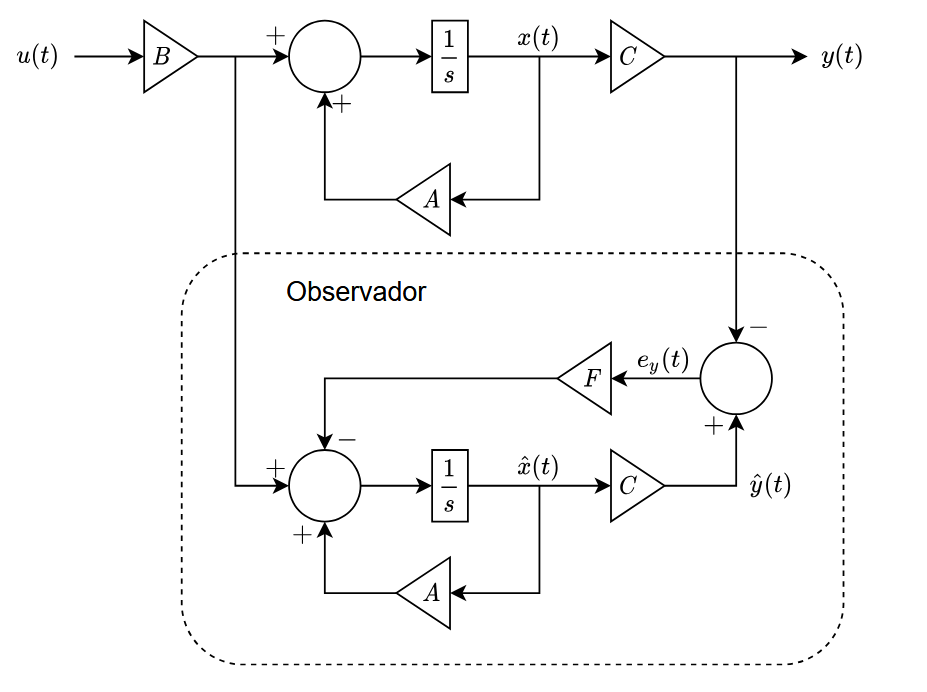
\includegraphics[width=.6\textwidth]{../figures/Auxiliar_4_3.png}
    \caption{El observador replica la ecuación $\dot{\hat x}=A\hat x + Bu + F(y-\hat y)$. La rama principal implementa el modelo del sistema ($A$, $B$ y el integrador). La rama vertical superior lleva la salida estimada $\hat y = C\hat x$ al comparador donde se obtiene el error de salida $e_y$. Ese error, tras el bloque de ganancia $F$, se suma como término corrector que desplaza los polos de la dinámica del error a posiciones elegidas (más rápidos), garantizando convergencia de $\hat x$ hacia $x$. De este modo el diseño de $F$ es independiente del de $K$, ilustrando el principio de separación.}
  \end{figure}

Tenemos que el gemelo digital vendra dado por
\begin{align}
\dot{\hat x} &= A\hat x + Bu + L\big(y-\hat y\big)\\
\hat y &= C\hat x,
\end{align}
con error de estimación $e:=x-\hat x$. Entonces
\begin{align}
\dot e
&= \dot x - \dot{\hat x}
= (Ax+Bu) - (A\hat x + Bu + L(y-\hat y)) \\
&= A(x-\hat x) - L\big(Cx - C\hat x\big)
= (A-LC)e. \label{eq:error_dyn}
\end{align}
Con lo que tenemos que:
\begin{align}
\dot e &= (A-LC)e,
\end{align}
Luego los polos del observador son los autovalores de $A-LC$, por lo que deberemos obtenerlos tal que se ubiquen en $-10$ y $-5$, por tanto:
\begin{align}
  L= \begin{bmatrix} \ell_1 \\ \ell_2 \end{bmatrix}\\
  LC = \begin{bmatrix} 0.01\ell_1 & 0 \\ 0.01\ell_2 & 0 \end{bmatrix}
\end{align}
De esta manera tenemos que:
\begin{align}
  \det(\lambda I - (A-LC)) &= \det\begin{bmatrix} \lambda + 2 + 0.01\ell_1 & -10 \\ 1 + 0.01\ell_2 & \lambda + 1 \end{bmatrix} \\
  &= (\lambda + 2 + 0.01\ell_1)(\lambda + 1) - (-10)(1 + 0.01\ell_2) \\
  &= \lambda^2 + (3 + 0.01\ell_1)\lambda + (12 + 0.01\ell_1 + 0.1\ell_2)
\end{align}
Dado que queremos ubicar los polos en $-10$ y $-5$, el polinomio característico deseado es:
\begin{align}
  (\lambda + 10)(\lambda + 5) = \lambda^2 + 15\lambda + 50
\end{align}
Igualando coeficientes, obtenemos el siguiente sistema de ecuaciones:
\begin{align}
  3 + 0.01\ell_1 &= 15 \\
  12 + 0.01\ell_1 + 0.1\ell_2 &= 50
\end{align}
Resolviendo el sistema, tenemos:
\begin{align}
  \ell_1 &= 1200 \\
  12 + 0.01(1200) + 0.1\ell_2 &= 50 \\
  12 + 12 + 0.1\ell_2 &= 50 \\
  24 + 0.1\ell_2 &= 50 \\
  0.1\ell_2 &= 26 \\
  \ell_2 &= 260
\end{align}
Con lo que finalmente tenemos que L sera:
\[
L=\begin{bmatrix}1200\\260\end{bmatrix}
\]
Con lo que finalmente se obtiene el observador deseado.
\end{solution}
\end{document}